\subsection{Open Graph Benchmark (OGB) - Biology}
{{\footnotesize
\noindent OGB-Biology is a suite of large-scale biological network datasets (protein-protein
interaction, drug-target, etc.) with standardized splits and evaluation protocols 
for node, link, and graph property prediction tasks.


\begin{description}[labelwidth=4cm, labelsep=1em, leftmargin=4cm, itemsep=0.1em, parsep=0em]
  \item[date:] 2020-05-02
  \item[version:] 1
  \item[last\_updated:] 2020-05-02
  \item[expired:] false
  \item[valid:] yes
  \item[valid\_date:] 2020-05-02
  \item[url:] \href{https://ogb.stanford.edu/docs/home/}{https://ogb.stanford.edu/docs/home/}
  \item[doi:] 10.48550/arXiv.2005.00687
  \item[domain:] Graph ML
  \item[focus:] Biological graph property prediction
  \item[keywords:]
    - node prediction
    - link prediction
    - graph classification
  \item[licensing:] MIT License
  \item[task\_types:]
    - Node property prediction
    - Link property prediction
    - Graph property prediction
  \item[ai\_capability\_measured:]
    - Scalability and generalization in graph ML for biology
  \item[metrics:]
    - Accuracy
    - ROC-AUC
  \item[models:]
    - GCN
    - GraphSAGE
    - GAT
  \item[ml\_motif:]
    - Chemical biology
  \item[type:] Benchmark
  \item[ml\_task:]
    - Supervised Learning
  \item[solutions:] 0
  \item[notes:] Community-driven updates
  \item[contact.name:] OGB Team
  \item[contact.email:] ogb@cs.stanford.edu
  \item[datasets.links.name:] OGB Webpage
  \item[datasets.links.url:] \href{https://ogb.stanford.edu/docs/dataset\_overview/}{https://ogb.stanford.edu/docs/dataset\_overview/}
  \item[results.links.name:] unknown
  \item[results.links.url:] \href{unknown}{unknown}
  \item[fair.reproducible:] True
  \item[fair.benchmark\_ready:] True
  \item[id:] open\_graph\_benchmark\_ogb\_-\_biology
  \item[Citations:] \cite{hu2021opengraphbenchmarkdatasets}
\end{description}

{\bf Ratings:} ~ \\

\begin{tabular}{p{0.15\textwidth} p{0.07\textwidth} p{0.7\textwidth}}
\hline
Rating & Value & Reason \\
\hline
dataset & 5 & Fully FAIR- datasets are versioned, split, and accessible via a standardized API; extensive metadata and documentation are included.
 \\
documentation & 5 & All necessary information is included in a paper.
 \\
metrics & 5 & Reproducible, quantitative metrics (e.g., ROC-AUC, accuracy) that are tightly aligned with the tasks.
 \\
reference\_solution & 3 & Multiple baselines implemented and documented (GCN, GAT, GraphSAGE). No contraints.
 \\
software & 5 & All necessary information is provided on the Github
 \\
specification & 4 & Tasks (node/link/graph property prediction) are clearly specified with input/output formats and standardized protocols; constraints (e.g., splits) are well-defined. No constraints.
 \\
\hline
\end{tabular}

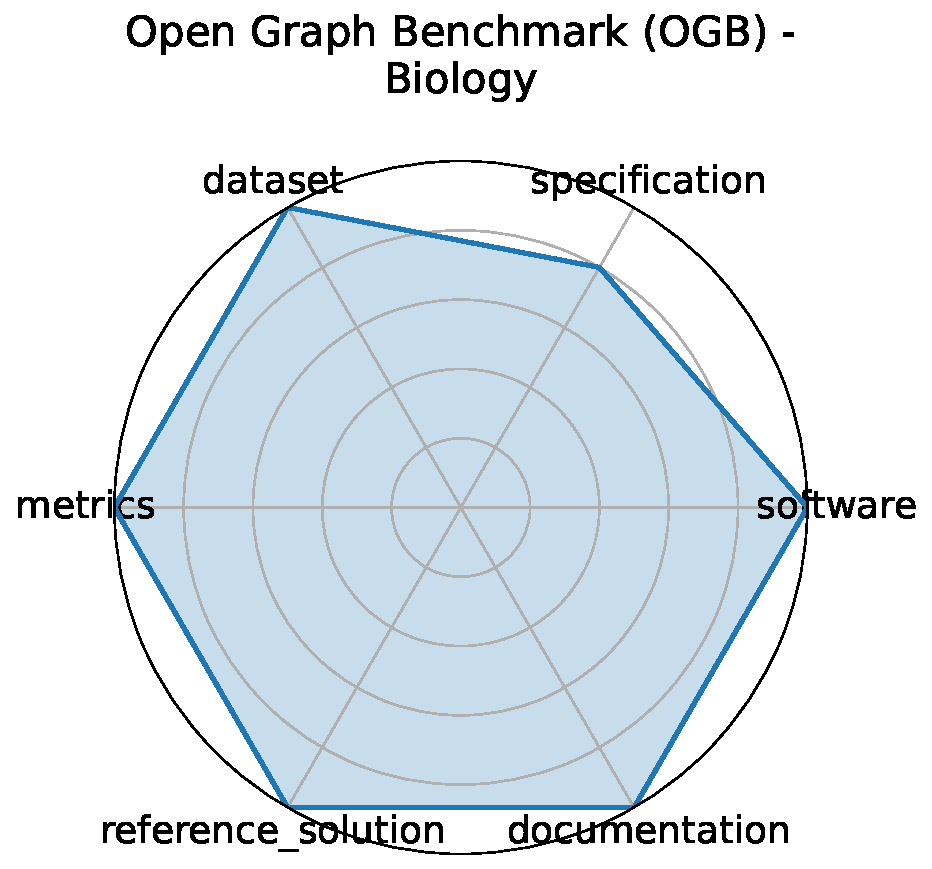
\includegraphics[width=0.2\textwidth]{open_graph_benchmark_ogb_-_biology_radar.pdf}
}}
\clearpage